%%%%%%%%%%%%%%%%%%%%%%%%%%%%%%%%%%%%%%%%%%%%%%%%%%%%%%%%%%%%%%%%%%%%%%
%%  Copyright by Wenliang Du.                                       %%
%%  This work is licensed under the Creative Commons                %%
%%  Attribution-NonCommercial-ShareAlike 4.0 International License. %%
%%  To view a copy of this license, visit                           %%
%%  http://creativecommons.org/licenses/by-nc-sa/4.0/.              %%
%%%%%%%%%%%%%%%%%%%%%%%%%%%%%%%%%%%%%%%%%%%%%%%%%%%%%%%%%%%%%%%%%%%%%%

\newcommand{\commonfolder}{../../common-files}

\documentclass[11pt]{article}

\usepackage[most]{tcolorbox}
\usepackage{times}
\usepackage{epsf}
\usepackage{epsfig}
\usepackage{amsmath, alltt, amssymb, xspace}
\usepackage{wrapfig}
\usepackage{fancyhdr}
\usepackage{url}
\usepackage{verbatim}
\usepackage{fancyvrb}
\usepackage{adjustbox}
\usepackage{listings}
\usepackage{color}
\usepackage{subfigure}
\usepackage{cite}
\usepackage{sidecap}
\usepackage{pifont}
\usepackage{mdframed}
\usepackage{textcomp}
\usepackage{enumitem}


% Horizontal alignment
\topmargin      -0.50in  % distance to headers
\oddsidemargin  0.0in
\evensidemargin 0.0in
\textwidth      6.5in
\textheight     8.9in 

\newcommand{\todo}[1]{
\vspace{0.1in}
\fbox{\parbox{6in}{TODO: #1}}
\vspace{0.1in}
}


\newcommand{\unix}{{\tt Unix}\xspace}
\newcommand{\linux}{{\tt Linux}\xspace}
\newcommand{\minix}{{\tt Minix}\xspace}
\newcommand{\ubuntu}{{\tt Ubuntu}\xspace}
\newcommand{\setuid}{{\tt Set-UID}\xspace}
\newcommand{\openssl} {\texttt{openssl}}


\pagestyle{fancy}
\lhead{\bfseries SEED Labs}
\chead{}
\rhead{\small \thepage}
\lfoot{}
\cfoot{}
\rfoot{}


\definecolor{dkgreen}{rgb}{0,0.6,0}
\definecolor{gray}{rgb}{0.5,0.5,0.5}
\definecolor{mauve}{rgb}{0.58,0,0.82}
\definecolor{lightgray}{gray}{0.90}


\lstset{%
  frame=none,
  language=,
  backgroundcolor=\color{lightgray},
  aboveskip=3mm,
  belowskip=3mm,
  showstringspaces=false,
%  columns=flexible,
  basicstyle={\small\ttfamily},
  numbers=none,
  numberstyle=\tiny\color{gray},
  keywordstyle=\color{blue},
  commentstyle=\color{dkgreen},
  stringstyle=\color{mauve},
  breaklines=true,
  breakatwhitespace=true,
  tabsize=3,
  columns=fullflexible,
  keepspaces=true,
  escapeinside={(*@}{@*)}
}

\newcommand{\newnote}[1]{
\vspace{0.1in}
\noindent
\fbox{\parbox{1.0\textwidth}{\textbf{Note:} #1}}
%\vspace{0.1in}
}


%% Submission
\newcommand{\seedsubmission}{You need to submit a detailed lab report, with screenshots,
to describe what you have done and what you have observed.
You also need to provide explanation
to the observations that are interesting or surprising.
Please also list the important code snippets followed by
explanation. Simply attaching code without any explanation will not
receive credits.}

%% Book
\newcommand{\seedbook}{\textit{Computer \& Internet Security: A Hands-on Approach}, 2nd
Edition, by Wenliang Du. See details at \url{https://www.handsonsecurity.net}.}

%% Videos
\newcommand{\seedisvideo}{\textit{Internet Security: A Hands-on Approach},
by Wenliang Du. See details at \url{https://www.handsonsecurity.net/video.html}.}

\newcommand{\seedcsvideo}{\textit{Computer Security: A Hands-on Approach},
by Wenliang Du. See details at \url{https://www.handsonsecurity.net/video.html}.}

%% Lab Environment
\newcommand{\seedenvironment}{This lab has been tested on our pre-built
Ubuntu 16.04 VM, which can be downloaded from the SEED website. }

\newcommand{\seedenvironmentA}{This lab has been tested on our pre-built
Ubuntu 16.04 VM, which can be downloaded from the SEED website. }

\newcommand{\seedenvironmentB}{This lab has been tested on our pre-built
Ubuntu 20.04 VM, which can be downloaded from the SEED website. }

\newcommand{\seedenvironmentAB}{This lab has been tested on our pre-built
Ubuntu 16.04 and 20.04 VMs, which can be downloaded from the SEED website. }

\newcommand{\nodependency}{Since we use containers to set up the lab environment, 
this lab does not depend too much on our SEED VM. You can do this lab
using other VMs or physical machines. }







\newcommand{\seedlabcopyright}[1]{
\vspace{0.1in}
\fbox{\parbox{6in}{\small Copyright \copyright\ {#1}\ \ by Wenliang Du.\\
      This work is licensed under a Creative Commons
      Attribution-NonCommercial-ShareAlike 4.0 International License.
      If you remix, transform, or build upon the material, 
      this copyright notice must be left intact, or reproduced in a way that is reasonable to
      the medium in which the work is being re-published.}}
\vspace{0.1in}
}





\newcommand{\rebindingFigs}{./Figs}

\lhead{\bfseries SEED Labs -- DNS Rebinding Attack Lab}


\begin{document}

\begin{center}
{\LARGE DNS Rebinding Attack Lab}
\end{center}

\seedlabcopyright{2019 - 2020}


\newcounter{task}
\setcounter{task}{1}
\newcommand{\tasks} {\bf {\noindent (\arabic{task})} \addtocounter{task}{1} \,}



% *******************************************
% SECTION
% ******************************************* 
\section{Introduction}


The objective of this lab is two-fold: (1) demonstrate how 
the DNS rebinding attack works, and (2) help students gain
the first-hand experience on how to use the DNS rebinding
technique to attack IoT devices. In the setup, we have a simulated IoT device, 
which can be controlled through
a web interface (this is typical for many IoT devices). Many IoT devices do not have 
a strong protection mechanism, if attackers can directly interact with them, they can
easily compromise these devices. 


The IoT device simulated in this lab is a thermostat, 
which controls the room temperature. 
To successfully set the temperature, the client needs to be able to interact with the
IoT server. Since the IoT device is behind the firewall, outside machines
cannot interact with the IoT device, and will therefore not be able to 
control the thermostat. To defeat the firewall protection, the attacking code must get into the 
internal network first. This is not difficult. Any time when a user from 
the internal network visits the attacker's website, the attacker's code (JavaScript
code) actually runs from the user's browser, and therefore runs inside the 
protected internal network. However, due to the sandbox protection implemented 
by browsers, the attacker's code still cannot interact with the IoT device, even though it 
is now inside the internal network. 


The objective of this lab is to use the DNS rebinding attack to 
circumvent the sandbox protection, so
the JavaScript code from the attacker can successfully get the 
essential information from the IoT device and then 
use the information to set the temperature 
of the thermostat to a dangerously high value. This lab covers the
following topics:

\begin{itemize}[noitemsep]
\item DNS server setup
\item DNS rebinding attack
\item Attacks on IoT devices
\item Same Origin Policy
\end{itemize}


\paragraph{Readings and videos.}
Detailed coverage of the DNS protocol and attacks can be found in the following:

\begin{itemize}
\item Chapter 18 of the SEED Book, \seedbook
\item Section 7 of the SEED Lecture, \seedisvideo
\end{itemize}


\paragraph{Lab environment.} \seedenvironmentC



%\vspace{0.2in}
%\noindent
%\fbox{\parbox{\textwidth}{
%\noindent
%\textbf{Customization.} 
%In this lab description, we use the domain \texttt{attacker32.com} to refer to the 
%domain controlled by the attacker. When students do this lab, they are not allowed 
%to use this domain name; instead, they should use a name that includes 
%their last names (the domain name is only used internally inside the VMs, so it does not 
%matter whether the name is owned by others or not). 
%The purpose of this requirement is to differentiate student's work.
%}}





% *******************************************
% SECTION
% ******************************************* 
\section{Background: IoT}

Our attack target is an IoT device behind the firewall. We cannot directly
access this IoT device from outside. Our goal is to get an inside
user to run our JavaScript code, so we can use
the DNS rebinding attack to interact with the IoT device.


Many IoT devices have a simple built-in web server, so users can
interact with these devices via web APIs. Typically, these IoT
devices are protected by a firewall, they cannot be accessed directly
from outside. Due to this type of protection,  many IoT devices do not
implement a strong authentication mechanism. If attackers can find ways
to interact with them, they can easily compromise its security.

We emulate such a vulnerable IoT device using 
a simple web server, which serves
two APIs: \texttt{password} and \texttt{temperature}.
The IoT device can set the room temperature. To do that,
we need to send out an HTTP request to the server's
\texttt{temperature} API; the request should include
two pieces of data: the target temperature value and a
password.  The password is a secret that changes
periodically, but it can be fetched using
the \texttt{password} API. Therefore, to successfully
set the temperature, users needs to
first get the password, and then attach the password
in the \texttt{temperature} API.

The password is not meant for the authentication purpose; it is used to defeat the Cross-Site
Request Forgery (CSRF) attack. Without this protection, a simple CSRF attack is sufficient;
there is no need to use the more sophisticated DNS rebinding attack.
For the sake of simplicity, we hardcoded the
password; in real systems, the password will be re-generated periodically.




% *******************************************
% SECTION
% ******************************************* 
\section{Lab Environment Setup Using Container}



\begin{figure}[htb]
\centering
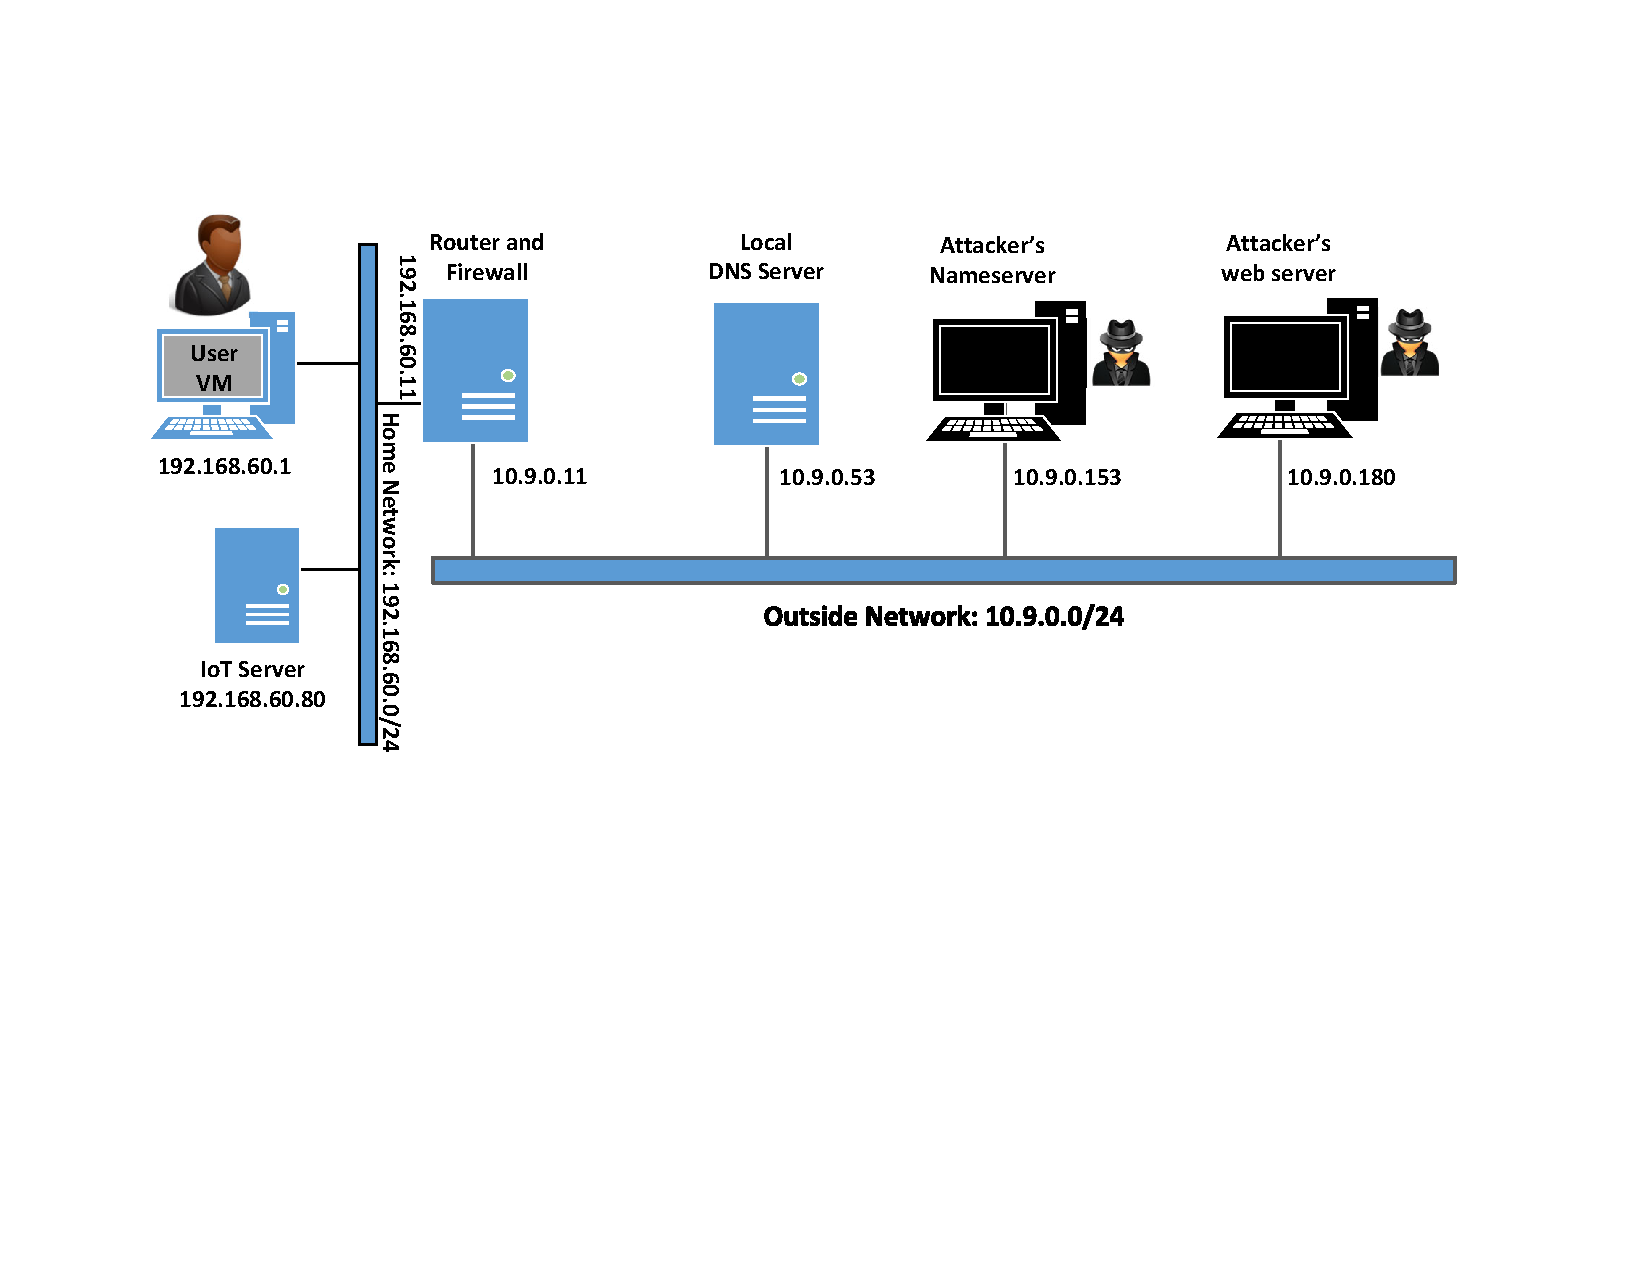
\includegraphics[width=0.9\textwidth]{\commonfolder/Figs/IoT_2lans.pdf}
\caption{Lab environment setup}
\label{rebind:fig:labsetup}
\end{figure}


In this lab, we will use six machines. 
The lab environment setup is illustrated
in Figure~\ref{rebind:fig:labsetup}. Only the user machine 
will be using VM, and the others are all containers. 
In the setup, we have two networks, a home network and 
an outside network. The home network 
simulates a typical network at home. 
The user machine and the IoT 
services are connected to this network, which
is protected by the firewall on the router container. 
The firewall blocks
all traffic going to the \texttt{192.168.60.80}. 
This way, outside machines cannot 
access the IoT device.
We also set up a NAT server on the router, so the machines
on the home network can access outside (and the reply
packets can come back). 

The second network simulates the outside world. In addition to
the router, there are three containers attached to this network,
one serving as the local DNS server, and the other two
serving as the attacker's nameserver and web server.
The attacker owns the \texttt{attacker32.com} domain, 
which is hosted by the attacker's nameserver container. 
The web server hosts a malicious website used for the 
attack. 



% -------------------------------------------
% SUBSECTION
% -------------------------------------------
\subsection{Container Setup and Commands}


%%%%%%%%%%%%%%%%%%%%%%%%%%%%%%%%%%%%%%%%%%%%
Please download the
\texttt{Labsetup.zip} file to your VM from the lab's website,
unzip it, enter the \texttt{Labsetup} folder, and 
use the \texttt{docker-compose.yml} file to 
set up the lab environment. Detailed explanation
of the content in this file and all the involved 
\texttt{Dockerfile} can be found from the 
user manual, which is linked to the website of this lab.
If this is the first time you set up a SEED lab environment
using containers, it is very important that you read 
the user manual. 

In the following, we list some of the commonly
used commands related to Docker and Compose. 
Since we are going to use 
these commands very frequently, we have created aliases for them
in the \texttt{.bashrc} file (in our provided SEEDUbuntu 20.04 VM).


\begin{lstlisting}
$ docker-compose build  # Build the container image
$ docker-compose up     # Start the container
$ docker-compose down   # Shut down the container

// Aliases for the Compose commands above
$ dcbuild       # Alias for: docker-compose build
$ dcup          # Alias for: docker-compose up
$ dcdown        # Alias for: docker-compose down
\end{lstlisting}


All the containers will be running in the background. To run
commands on a container, we often need to get a shell on
that container. We first need to use the \texttt{"docker ps"}  
command to find out the ID of the container, and then
use \texttt{"docker exec"} to start a shell on that 
container. We have created aliases for them in
the \texttt{.bashrc} file.

\begin{lstlisting}
$ dockps        # Alias for: docker ps --format "{{.ID}}  {{.Names}}" 
$ docksh <id>   # Alias for: docker exec -it <id> /bin/bash

# The following example shows how to get a shell inside hostC
$ dockps
b1004832e275  hostA-10.9.0.5
0af4ea7a3e2e  hostB-10.9.0.6
9652715c8e0a  hostC-10.9.0.7

$ docksh 96
root@9652715c8e0a:/#  

# Note: If a docker command requires a container ID, you do not need to 
#       type the entire ID string. Typing the first few characters will 
#       be sufficient, as long as they are unique among all the containers. 
\end{lstlisting}


If you encounter problems when setting up the lab environment, 
please read the ``Common Problems'' section of the manual
for potential solutions.


%%%%%%%%%%%%%%%%%%%%%%%%%%%%%%%%%%%%%%%%%%%%



% -------------------------------------------
% SUBSECTION
% ------------------------------------------- 
\subsection{Configure the User VM}

We need to provide further configuration on the user VM.


\paragraph{Step 1. Reduce Firefox's DNS caching time.}
To reduce load on DNS servers and to speed up response time, Firefox browser caches DNS
results.  By default, the cache's expiration time is 60 seconds. That means that our DNS
rebinding attack needs to wait for at least 60 seconds. To make our life easier, we reduce
the time to 10 seconds or less. Type \texttt{about:config} in the URL field.
After clicking through a warning page, we will see a list of preference names and their values.
Search for \texttt{dnsCache}, find the following entry and change its value:

\begin{lstlisting}
(*@\textbf{network.dnsCacheExpiration}@*):  change its value to 10 (default is 60)
\end{lstlisting}

After making the change, we should exit from the Firefox browser, and restart it; otherwise the
change will not take effect.


\paragraph{Step 2. Change \texttt{/etc/hosts}.}
We need to add the following entry to the \texttt{/etc/hosts} file. 
We will use \texttt{www.seedIoT32.com} as the name for the 
IoT server. Its IP address is \texttt{192.168.60.80}. 
We need to use the superuser privilege to modify this file (using \texttt{sudo}): 

\begin{lstlisting}
192.168.60.80  www.seedIoT32.com
\end{lstlisting}

While we are in this file, check whether there is any entry 
that contains \texttt{attacker32.com}. Remove them if there 
is any. These entries may have been added when we worked on
other SEED labs, and their existence will cause problems for this lab. 


We can now test the IoT server. Point the browser to the following URL on the 
user VM. If everything is set up correctly, we should be able to see 
a thermostat. We can also change the temperature setting by dragging the 
sliding bar. Please provide a screenshot in your lab report. 

\begin{lstlisting}
http://www.seedIoT32.com
\end{lstlisting}
 


\paragraph{Step 3. Local DNS Server.}
We need to get the user VM to use a particular local DNS server. This is achieved by
setting the local DNS server as the first \texttt{nameserver} entry in the resolver
configuration file (\texttt{/etc/resolv.conf}). 
One challenge is that the provided VM uses the
Dynamic Host Configuration Protocol (DHCP) to obtain network configuration parameters, such as
IP address, local DNS server, etc. DHCP clients overwrite the \texttt{/etc/resolv.conf}
file with the information provided by the DHCP server.

One way to get our information into \texttt{/etc/resolv.conf} without worrying about
the DHCP is to add the following entry to the \path{/etc/resolvconf/resolv.conf.d/head}
file (\texttt{10.9.0.53} is the IP address of the local DNS server in our setup):

\begin{lstlisting}
nameserver 10.9.0.53
\end{lstlisting}

The content of the head file will be prepended to the dynamically generated resolver
configuration file. Normally, this is just a comment line (the comment in
\texttt{/etc/resolv.conf} comes from this head file). After making the change,
we need to run the following command for the change to take effect: 

\begin{lstlisting}
$ sudo resolvconf -u
\end{lstlisting}




% -------------------------------------------
% SUBSECTION
% ------------------------------------------- 
\subsection{Testing the Lab Setup.}

After configuring the user VM, use the \texttt{dig} command
to get the IP address of \texttt{www.attacker32.com}
and \texttt{ns.attacker32.com}. You should get 
\texttt{10.9.0.180} and \texttt{10.9.0.153}, respectively. 
If you do not get this, your lab environment is not 
set up correctly. 


We can now test the attacker's website. 
Point the browser to the following URL on the user VM, and you should 
be able to see the attacker's website. 
Please provide a screenshot in your lab report. 

\begin{lstlisting}
http://www.attacker32.com
\end{lstlisting}

\paragraph{Note.} We may have used the same hostname  
\texttt{www.attacker32.com} in other SEED labs, so it is likely 
that this name is already mapped to a different IP address. Therefore,
if you do not see the expected attacker's website, you should 
check the \texttt{/etc/hosts} file, and remove
any entry that contains \texttt{attacker32.com}. 




% *******************************************
% SECTION
% ******************************************* 
\section{Launch the Attack on the IoT Device}

We are ready to launch the attack on the IoT device. To help students 
understand how the attack works, we break down
the attack into several incremental steps. 


% -------------------------------------------
% SUBSECTION
% ------------------------------------------- 
\subsection{Task 1. Understanding the Same-Origin Policy Protection}

In this task, we will do some experiment to understand the 
same-origin policy protection implemented on browsers. On the user VM,
we will browse the following three URLs. It is better to show these three pages on three
different Firefox windows (instead of on three different tabs), so they are all visible. 


\begin{lstlisting}
URL 1:  http://www.seedIoT32.com
URL 2:  http://www.seedIoT32.com/change
URL 3:  http://www.attacker32.com/change
\end{lstlisting}

 
The first page lets us see the current temperature setting of the thermostat (see
Figure~\ref{rebinding:fig:webpages}.a); it fetches
the temperature value from the IoT server once every second. We should keep this page always
visible, so we can see the temperature setting on the thermostat. 
The second and third pages
are identical (see Figure~\ref{rebinding:fig:webpages}.b), 
except that one comes from the IoT server, and the other comes from
the attacker's server. When we click the button on both pages, 
a request will be sent out to the IoT server to set its temperature. 
We are supposed to raise the thermostat's temperature 
to \texttt{99} Celsius.  


\begin{figure}[htb]
\begin{center}
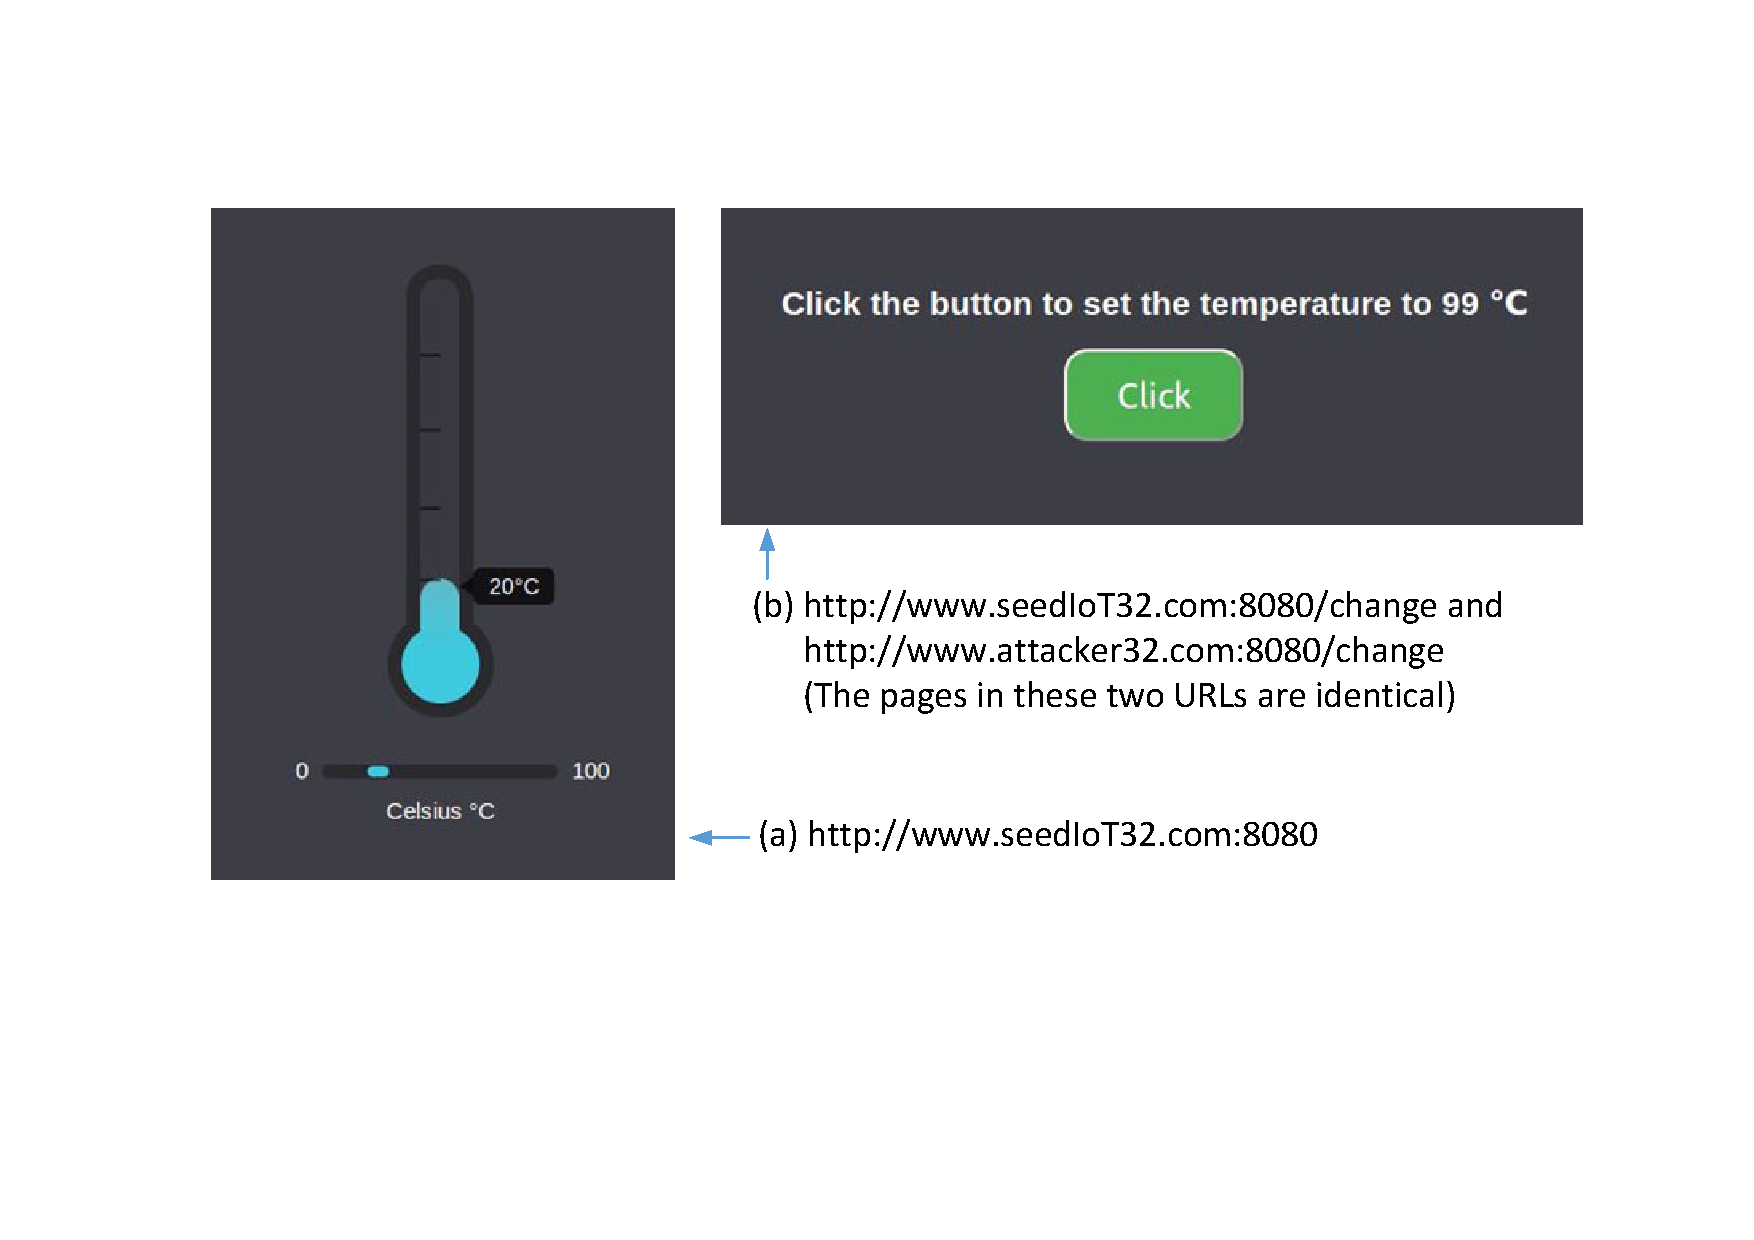
\includegraphics[width=0.8\textwidth]{\rebindingFigs/iot_webpages.pdf}
\end{center}
\caption{The web pages from the three URLs}
\label{rebinding:fig:webpages}
\end{figure}
 

Click the button on the second and third pages, and describe your observation. Which page
can successfully set the thermostat's temperature? Please explain why. 
To find the reason, click the following menu sequence from Firefox. A console window will appear,
which displays error messages if any. Hint: the reason is related to the same-origin policy 
enforced by browsers. Please explain why this policy causes one of the pages to fail.
 
\begin{lstlisting}
Web Developer -> Web Console
\end{lstlisting}
  


% -------------------------------------------
% SUBSECTION
% ------------------------------------------- 
\subsection{Task 2. Defeat the Same-Origin Policy Protection}


From the previous task, it seems impossible to
set the thermostat's temperature from the attacker's
page, due to the browser's   
same-origin policy protection.  The objective of this task
is to defeat such a protection, so we can set the 
temperature from this page. 


The main idea for defeating the same origin protection 
comes from the fact that the policy enforcement is 
based on the host name, not on the IP address, so as long as 
we use \texttt{www.attacker32.com} in the URL, we are complying with
the SOP policy, but that does not mean we are restricted 
to communicate with the \texttt{www.attacker32.com} web server.  


Before the user's browser sends out requests to \texttt{www.attacker32.com},
it first needs to know the IP address of \texttt{www.attacker32.com}. 
A DNS request will be sent out from the user's machine. If the 
IP address is not cached at the local DNS server, a DNS request will
eventually be sent to \texttt{attacker32.com}'s  nameserver, which 
is controlled by the attacker. 
Therefore, the attacker can decide what to put in the response. 


\paragraph{Step 1: Modify the JavaScript code.}
On the attacker's web server, the JavaScript code running inside the 
\url{www.attacker32.com/change} page is 
stored in the following file: 
\path{/app/rebind_server/templates/js/change.js}. Since this page
comes from the \texttt{www.attacker32.com} server, 
according to the same-origin policy, it can only
interact with the same server. Therefore, we need to change the first 
line of the code from \url{http://www.seediot32.com} 
to the following (we have installed a simple editor called \texttt{nano}
in the container):

\begin{lstlisting}
let url_prefix = 'http://www.attacker32.com'
\end{lstlisting}
 

After making the change, restart the attacker's web server container (see the 
command below). Then go to the user VM, refresh the page, and click the button again. 
Do you still see the error
message in the web console? Please explain your observation. 


\begin{lstlisting}
$ docker ps
...
78359039627a  attacker-www-10.9.0.180

$ docker container restart 7835
\end{lstlisting}
 


\paragraph{Step 2: Conduct the DNS rebinding.}
Our JavaScript code sends requests to \url{www.attacker32.com}, 
i.e., the requests will come back to the Attacker's web server. That is not 
what we want; we want the requests to go to the IoT server. 
This can be achieved using the DNS rebinding 
technique. We first map \url{www.attacker32.com} to the IP address of the attacker's
web server, so
the user can get the actual page from \url{http://www.attacker32.com/change}. 
Before we click on the button on the page, we remap
the \url{www.attacker32.com} hostname to the IP address of the IoT server, so
the request triggered by the button will go to the IoT server. That is exactly what 
we want. 


To change the DNS mapping, students can modify the 
\path{zone_attacker32.com} file inside attacker's nameserver container.
The zone file can be found in 
the \texttt{/etc/bind} folder. 
The following shows the content of the zone file. The first 
entry is the default Time-To-Live (\texttt{TTL}) value (seconds) 
for the response, specifying how long the response can stay in
the DNS cache. This value may need to be modified. 
The following is the content of the zone file:

\begin{lstlisting}
$TTL 1000
@       IN      SOA   ns.attacker32.com. admin.attacker32.com. (
                2008111001
                8H
                2H
                4W
                1D)

@       IN      NS    ns.attacker32.com.

@       IN      A     10.9.0.22
www     IN      A     10.9.0.22
ns      IN      A     10.9.0.21
*       IN      A     10.9.0.22
\end{lstlisting}


After making the changes to the zone file, 
run the following command to ask the nameserver 
to reload the revised zone data. 

\begin{lstlisting}
# rndc reload attacker32.com
\end{lstlisting}



Because of the tasks conducted previously, the DNS mapping for the 
\texttt{www.attacker32.com} has already been cached by the local
DNS server, it will not expire until 1000 seconds later.  To 
shorten the waiting, students are allowed to clean out the cache using the 
following command (on the local DNS server). However, this can only be 
conducted before the attack starts. Once the attack starts, students 
are not allowed to touch the local DNS server. 

\begin{lstlisting}
// Do it on the local DNS server container
# rndc flush
\end{lstlisting}
 
 
If both steps in this task are done correctly, clicking the button 
on the \texttt{change} page from \url{www.attacker32.com} should be able to change
the thermostat's temperature successfully. Please provide evidence in your report to
demonstrate your success.


% -------------------------------------------
% SUBSECTION
% ------------------------------------------- 
\subsection{Task 3. Launch the Attack}

In the previous task, the user has to click the button to set the 
temperature to the dangerously high value. Obviously, it is unlikely that users will 
do that.  In this task, we need to do that automatically. We have already created 
a web page for that purpose. It can be accessed using the following URL:


\begin{lstlisting}
http://www.attacker32.com
\end{lstlisting}
 

Once you have loaded this page into the user VM, you should be able to see a page with a 
timer, which goes down from 10 to 0. Once it reaches 0, the JavaScript code 
on this page will send the set-temperature request to 
\url{http://www.attacker32.com}, and then reset the timer value to 10. 
Students need to use the DNS rebinding technique, so
once the timer reaches 0, the thermostat's temperature is set to 
88 Celsius. 



% *******************************************
% SECTION
% *******************************************
\section{Submission}

%%%%%%%%%%%%%%%%%%%%%%%%%%%%%%%%%%%%%%%%

You need to submit a detailed lab report, with screenshots,
to describe what you have done and what you have observed.
You also need to provide explanation
to the observations that are interesting or surprising.
Please also list the important code snippets followed by
explanation. Simply attaching code without any explanation will not
receive credits.

%%%%%%%%%%%%%%%%%%%%%%%%%%%%%%%%%%%%%%%%



\end{document}
